Recovery and downblending of \gls{HEU} to produce \gls{HALEU} means that 
the fuel contains impurities present in the original
\gls{HEU}. Known impurities in potential \gls{HEU}
supplies to create \gls{HALEU} include $^{232}$U and $^{236}$U
\cite{vaden_isotopic_2018,nelson_foreign_2010},  
which are parasitic neutron absorbers and have the potential to affect 
reactor physics and reactor operation. To investigate the magnitude of this 
effect, this chapter presents models of the use of 
impure \gls{HALEU} fuel in a reactor and compares it to the use of pure 
\gls{HALEU} (only $^{235}$U and $^{238}$U)
to understand how the impurities affect the performance of the reactor.
This chapter of work explores how the fuel affects the reactors, while 
the other chapters explore how the reactors affect the fuel cycle. We chose 
the downblended \gls{HALEU} compositions from these sources because
they are publicly available. 




ASTM has standards on UOX/MOX purity -- ASTM C776-06, C753 (2004), C757 (2006a)

\section{Methodology}
Full core models of Xe-100-like and \gls{MMR}-like were created in Serpent 
\cite{leppanen_serpent_2014} to model the neutronics and depletion of 
each reactor design. Each model was run using the ENDF VII.1 library
\cite{chadwick_endfb-vii1_2011}. The core geometries used are not 
the exact geometries used for each reactor, but are replications based 
on publicly-available information. 

We used the Sanagmon200 model from \cite{richter_isotopic_2022}, shown in 
Figure \ref{fig:xe100_core}, to serve as an Xe-100-like 
core model. The model itself can be found at \cite{richter_zoerichterphlox_2022}.
The Sangamon200 model is a pebble-bed, \gls{HTGR}-style reactor core model 
initially created to characterize the isotopic compositions and 
reactor physics of a pebble-bed, \gls{HTGR}. While this reactor model 
is very similar to current published data for the X-energy Xe-100
\cite{mulder_overview_2021}, there are some notable differences that affect 
the reactor physics. The first difference is that the \gls{TRISO} particles 
in the Sangamon200 are modeled as a blended mix of the \gls{TRISO} 
materials, not the explicit layers. Using a homogenized \gls{TRISO} particle 
decreases the \keff of the core by 4.45\%, but it does not reduce the 
neutron flux outside of error \cite{richter_isotopic_2022}. Despite 
the effect on \keff of this modeling decision, we continued to use the 
homogenized model of the \gls{TRISO} pebbles to be consistent with the 
published results of the Sanagamon200 \cite{richter_isotopic_2022}. 

The second 
notable difference is the reactor vessel shape. The Sanagmon200 is a simple 
cylinder, while the Xe-100 is a cylinder with a cone at the bottom to funnel 
the pebbles to a single point as they come out of the core. We do not account 
for any pebble movement within the core, so the geometry difference between 
the two cores should produce a negligible effect on the performance of the 
core as a whole.

\begin{figure}
    \centering 
    \begin{subfigure}{0.45\textwidth}
        \centering 
        \includegraphics[scale=0.03]{htgr-mr-full-core.inp_geom1.png}
        \caption{Radial view of Xe-100 core model.}
        \label{fig:xe100_core_radial}        
    \end{subfigure}
    \hfill
    \begin{subfigure}{0.45\textwidth}
        \centering 
        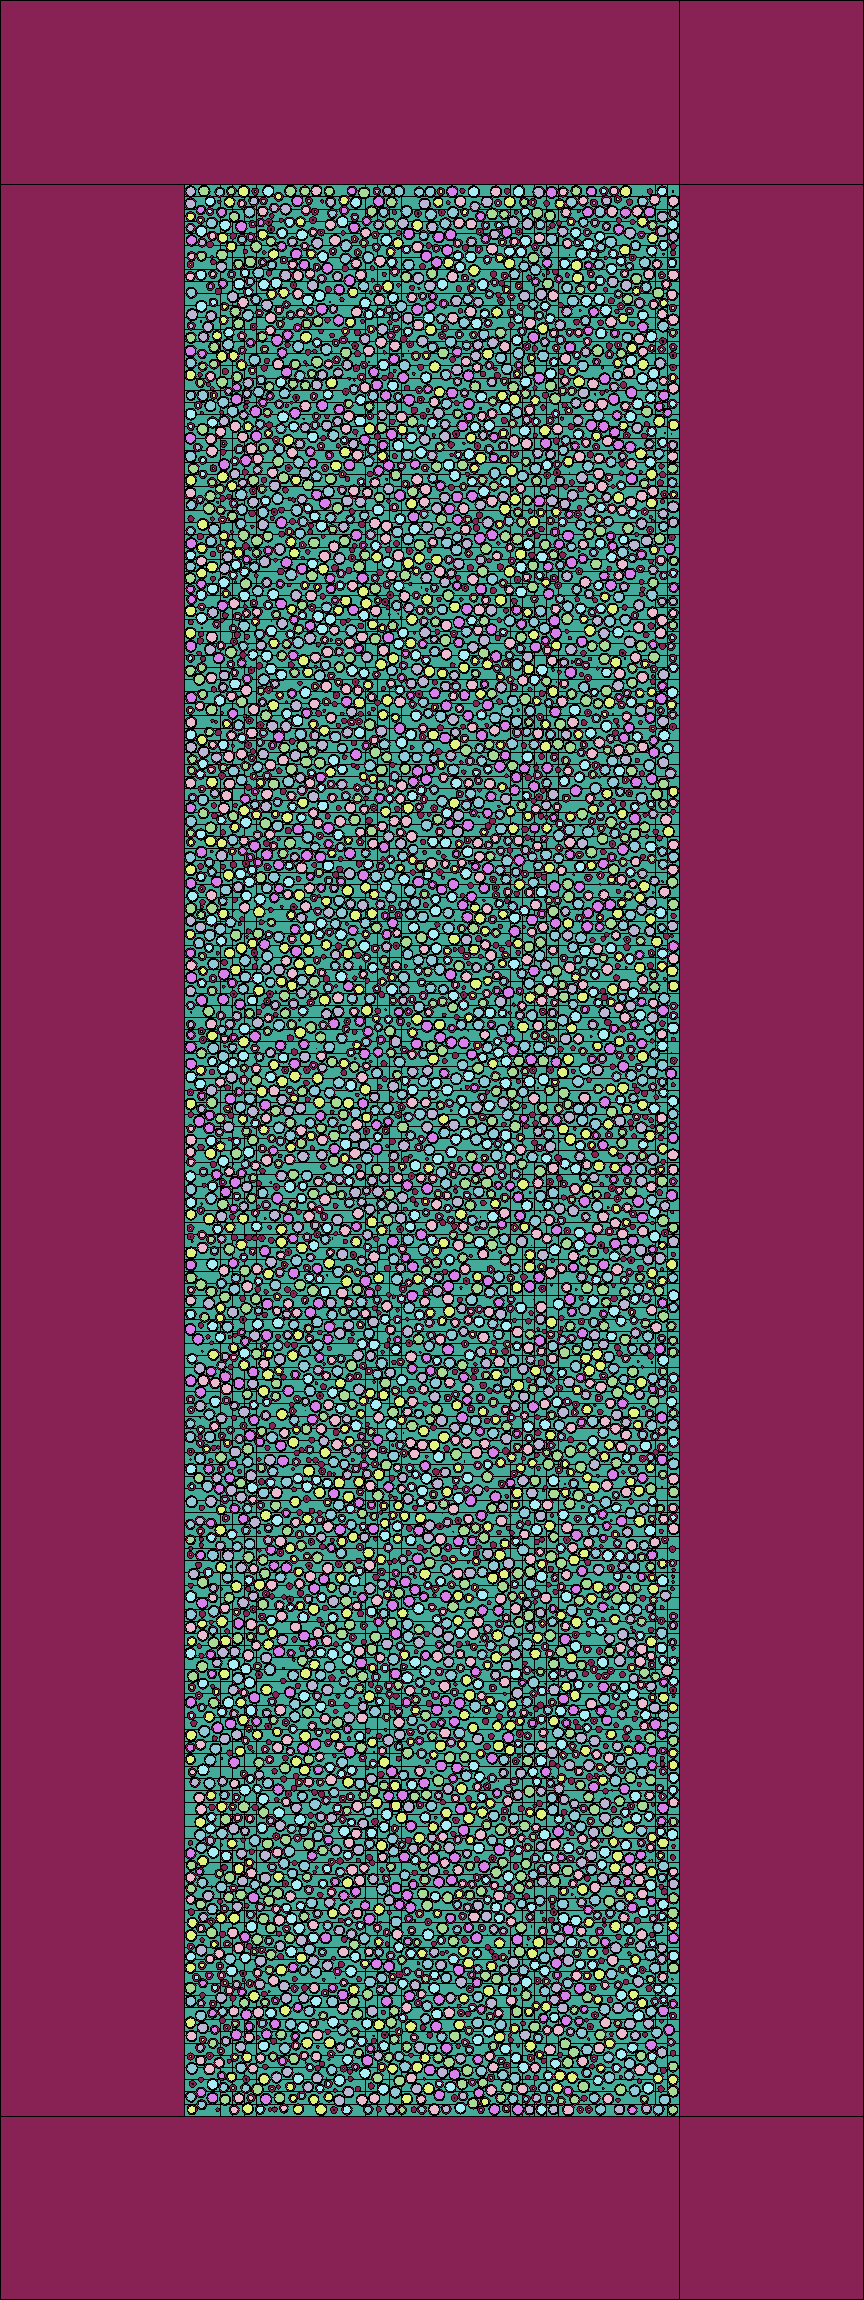
\includegraphics[scale=0.12]{htgr-mr-full-core.inp_geom3.png}
        \caption{Axial view of Xe-100 core model.}
        \label{fig:xe100_core_axial}        
    \end{subfigure}
    \caption{Xe-100 core model made in serpent.}
    \label{fig:xe100_core}
\end{figure}

Each \gls{TRISO} pebble in the core goes through multiple passes, an average 
of six passes per pebble. To account for the different burnup of 
the pebbles in an equilibrium core, the \gls{TRISO} pebble compositions are 
varied to reflect the composition of a pebble after it has gone through 
each number of passes. Each composition is stagnant, 
but the variations in 
compositions within a single pass would likely not cause significant 
changes in the isotopic composition of the fuel. 

The Sangamon200 is modeled an an isothermal state at 800 K \cite{richter_isotopic_2022}.
This model was run with 100,000 particles per cycle, 50 inactive cycles, 
and 150 active cycles. We did not perform depletion on the Sangamon200 model 
because our model 
does not capture the continuous refueling scheme used by the Xe-100 or 
any pebble movement. Performing depletion without modeling pebble movement 
would create non-physical differences from the equilibrium condition of 
this reactor model. Therefore, the results of this model will be comparisons
of the different uranium compositions for a single burnup step.

In order to update the fuel compositions, we calculated the correct 
isotopics for the enrichment level required tby this

We created an \gls{MMR}-like model primarily based on information in 
\cite{hawari_development_2018}, and supplemented or modified based on 
information published by \gls{USNC}. Information about the \gls{TRISO} 
particle and \gls{FCM} pellets was found in \cite{noauthor_usnc_2021}
and information about the graphite block dimensions and configuration 
was found via visual inspection of figures in \cite{venneri_micro_2019}. 
The final core configuration 
is different than what is modeled in \cite{hawari_development_2018} 
because the model by Hawari and Venneri is only meant to operate 
for 10 years, while the \gls{MMR} is meant to operate for 20 years. We 
selected this core configuration after modeling some of the other core 
configurations found in literature, and determining that this core 
configuration can operate the longest before going subcritical. 

Figure \ref{fig:mmr_core} shows the radial and axial geometry of the 
\gls{MMR} model. The fuel channels have a radius of 1.15 cm, the same
size as the \gls{FCM} pellets, the coolant channels have a radius of 
3 cm, arbitrarily chosen because no specific information was found, 
and the control rod channels have a radius of 6 cm, obtained from 
\cite{hawari_development_2018}. The \gls{TRISO} particles are modeled 
with a 40\% packing fraction in the \gls{FCM} particles
Control rods and burnable poisons are not included in this model, or 
the Sangamon200 model, so the control rod locations are modeled as 
filled with helium. There are five layers of the graphite compacts 
stacked to form the entire core, to approximate the number of 
fuel blocks described in \cite{noauthor_usnc_2021}. The entire core 
is assumed to be in an isothermal state at 800 K. There is a 20 cm 
thick graphite reflector above and below the stacks of graphite, 
and a 10 cm beryllium-oxide reflector on the outside of the 
graphite blocks of the core. Both of these reflectors are specified 
in \cite{hawari_development_2018}, with the thickness of the 
beryllium-oxide reflector given. However, the thickness of the graphite 
reflectors above and below the core was not specified, so we selected 
20 cm to prove 3-5 mean free paths of material. 
The input files for this model can be found at \textbf{create zenodo 
object}.

\begin{figure}
        \begin{subfigure}{0.48\textwidth}
                \centering
                
\includegraphics[scale=0.1]{bachmann-mmr_geom1.png}
                \caption{Radial view of the USNC MMR model.}
                \label{fig:mmr_radial}
        \end{subfigure}
        \hfill 
        \begin{subfigure}{0.48\textwidth}
                \centering
                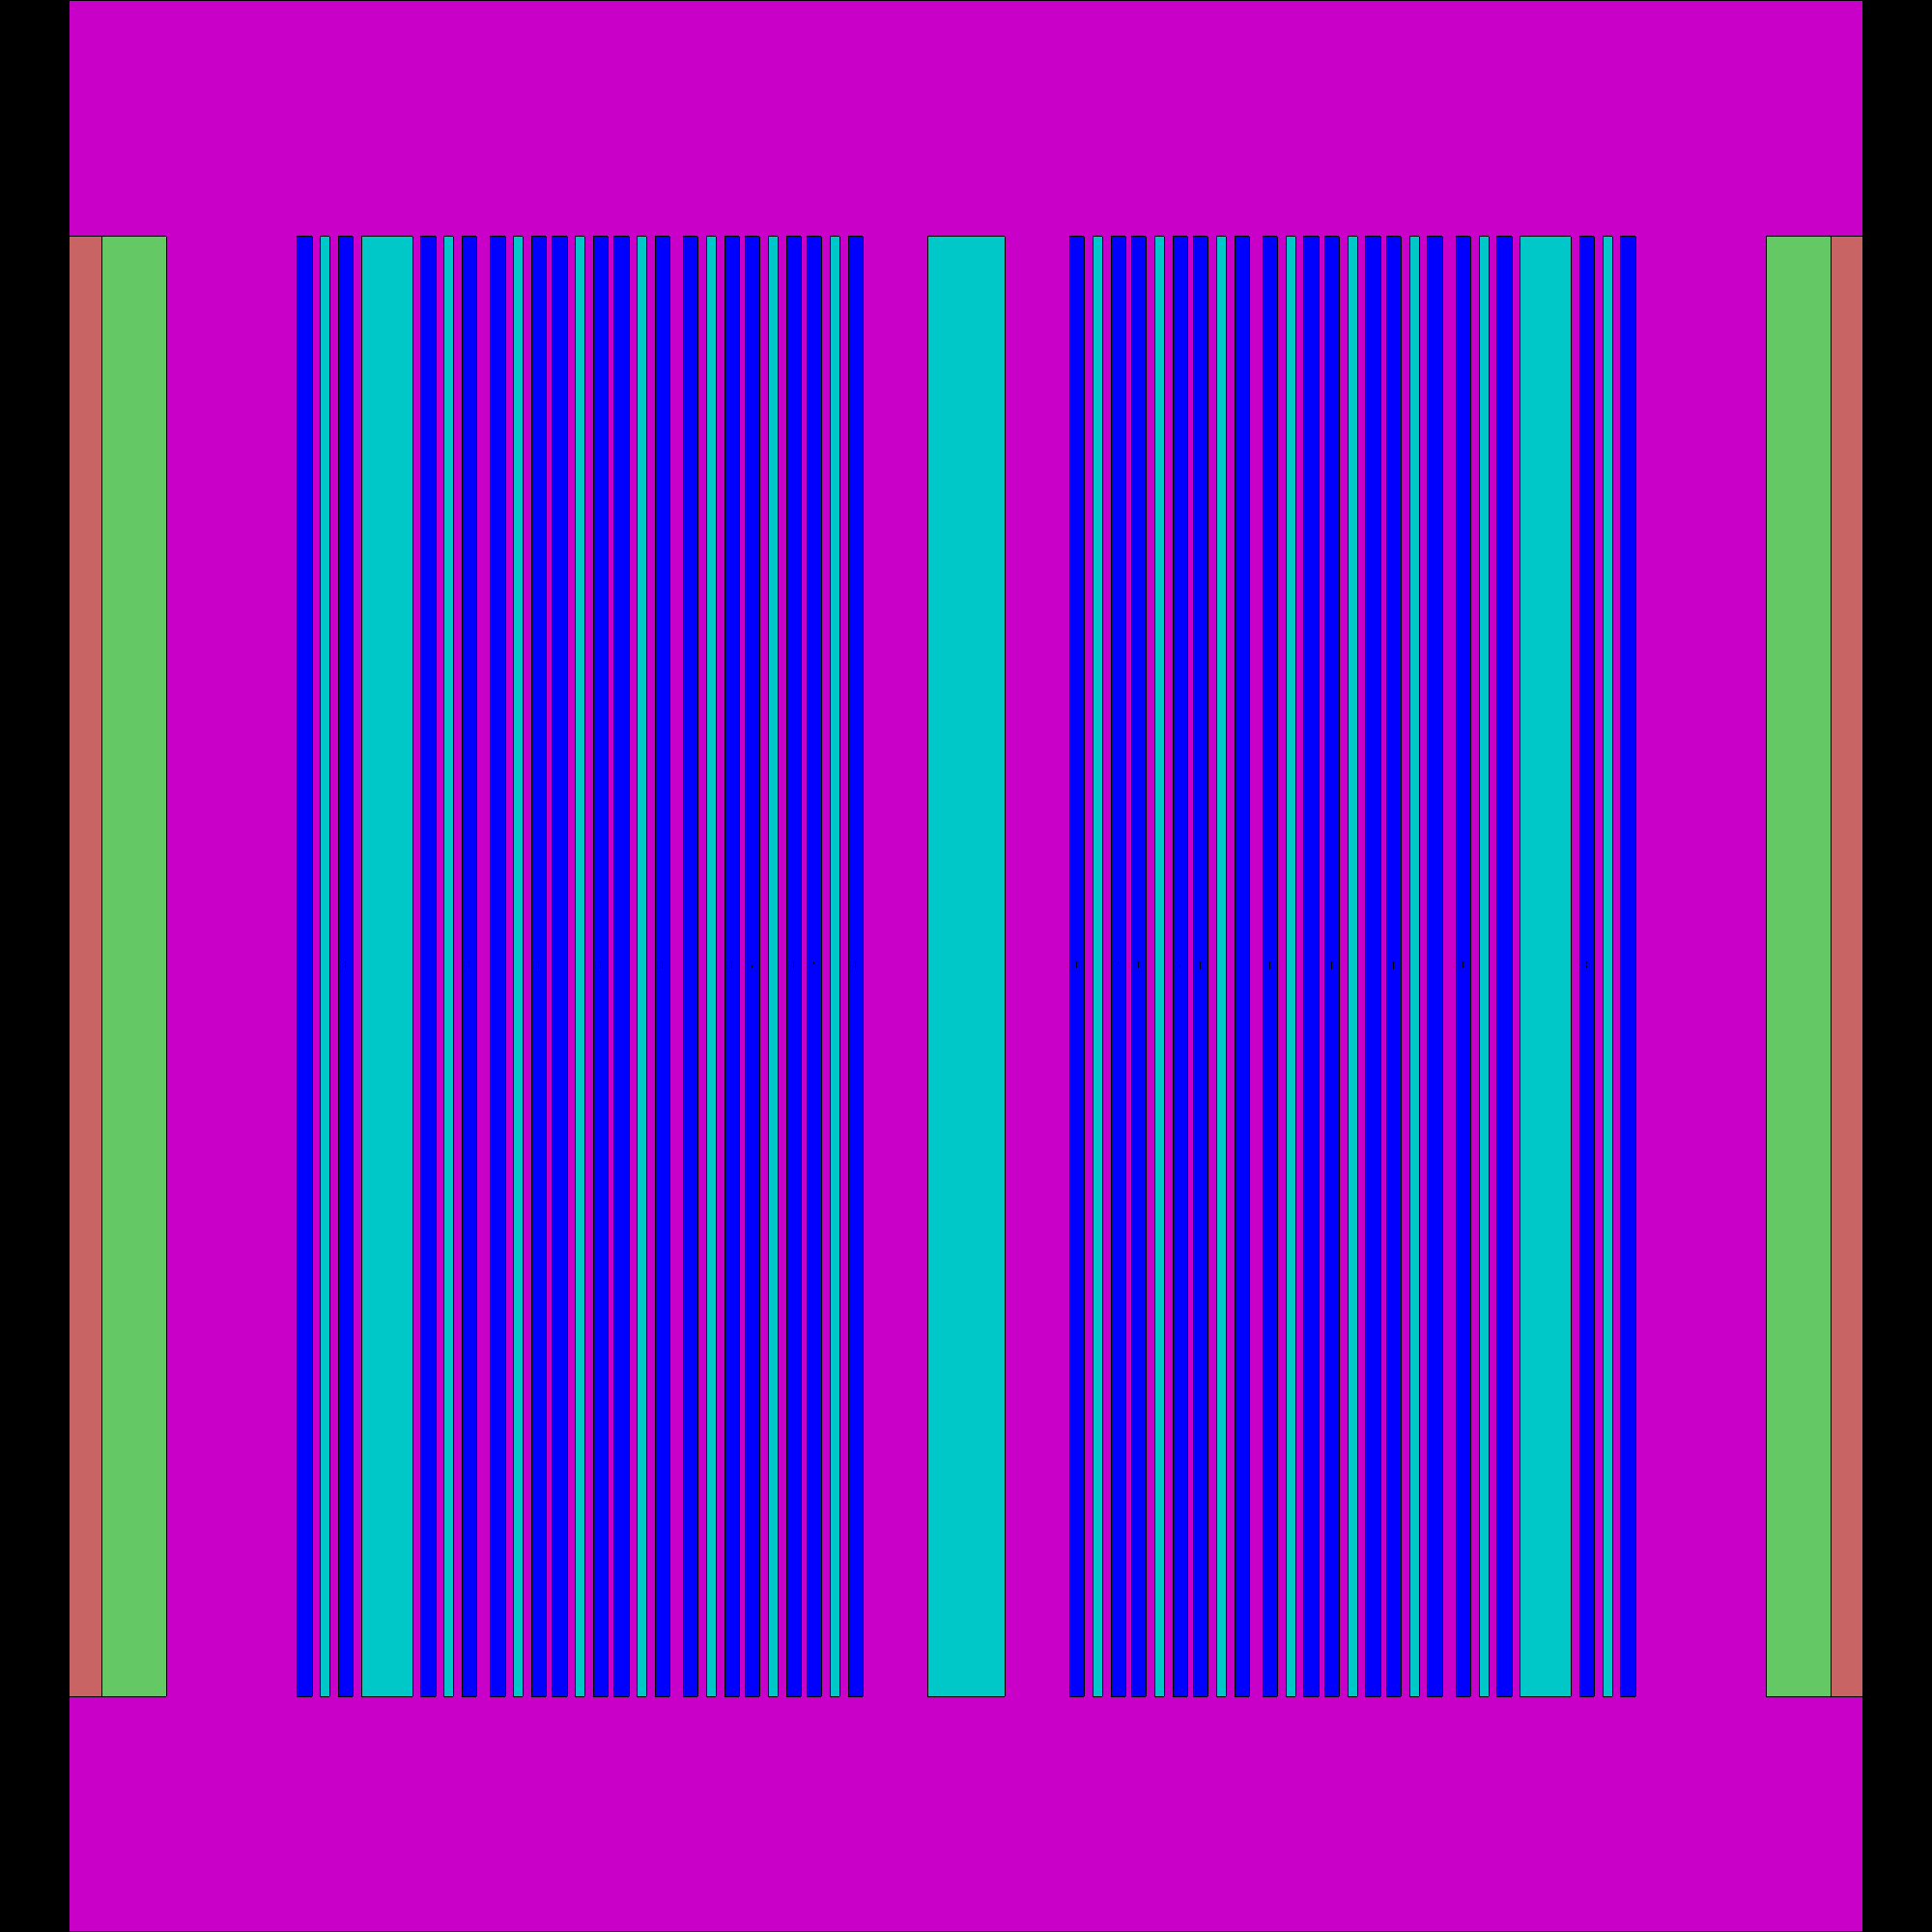
\includegraphics[scale=0.1]{bachmann-mmr_geom3.png}
                \caption{Axial view of the USNC MMR model.}
                \label{fig:mmr_axial}
        \end{subfigure}
        \caption{Geometry of USNC MMR-like core model in Serpent. The 
        light blue is helium, dark blue are fuel channels with TRISO particles, 
        and the bright pink is graphite in the core.}
        \label{fig:mmr_core}
\end{figure}

For the \gls{MMR}-like model we modeled depletion of the core across the 
expected 20 year lifetime of the \gls{MMR}, because the core is not 
meant to undergo refueling during those 20 years. Because we modeled 
depletion for this model, the flux, \keff, and temperature feedback coefficients
are compared at the \gls{BOL}, mid-cycle, and \gls{EOL} for the \gls{MMR}-like 
model. 

For both reactor models, we varied the fuel, coolant, and moderator temperatures 
between 750 K, 800 K, and 850 K to calculate the fuel, coolant, moderator, and 
total temperature feedback coefficients. We assumed a linear relationship between 
\keff and temperature to calculate the feedback coefficients. When varying the 
temperatures, we also varied the density of the materials. We calculated the 
density of the UO$_2$ by using the empirical relationship between density and 
temperature defined in \cite{fink_thermophysical_2000}. The calculated 
densities were assumed to hold true for the Sangamon200. 

We calculated the 
graphite density by linearly extrapolating from the data available in 
\cite{mceligot_thermal_nodate}. We calculated the density of the helium 
by interpolating on the data available in \cite{petersen_properties_nodate}, 
assuming the 3 MPa coolant pressure in the \gls{MMR}-like model as defined 
by \cite{noauthor_usnc_2021} and the 6 MPa inlet pressure defined in 
\cite{mulder_overview_2021}. 

\section{Results}
The points of comparison for this work include:
\begin{itemize}
        \item Neutron flux 
        \item \keff 
        \item \betaEff
        \item Temperature feedback coefficients
\end{itemize}

For the Sangamon200, these metrics are only compared for the initial 
state of the reactor. For the \gls{MMR}-like reactor these metrics 
are compared at \gls{BOL}, mid-cycle, and \gls{EOL}. Each metric provides a 
measurement of the performance of 
the reactor, such as the materials degradation rate, amount of burnable 
poisons required, control rod worth, and the cycle time. Investigating 
each of these results helps to determine if the impurities potentially 
present in \gls{HALEU} will prevent any of the design criteria of the 
reactors from being met. 

\subsection{Xe-100 reactor}

\subsubsection{\keff}
Table \ref{tab:xe100_keff} reports the \keff value when using each fuel 
composition. the impure fuels result in a slightly higher \keff 
than the pure fuel. The uranium isotopes mostly present in 
each of the fuel compositions (weight fraction of at least 1$\times 10^{-3}$)
are $^{234}$U, $^{235}$U, $^{236}$U, and $^{238}$U. The $^{235}$U weight 
fraction is the same in each fuel composition, so the impurities are 
displacing the $^{238}$U in the fuel. $^{234}$U and $^{236}$U have larger 
total fission cross sections than $^{238}$U, so their displacement of the
$^{238}$U in the fuel increases the neutron multiplication of the reactor. 
This is supported by the impure fuels leading to a slight increase 
in the $\eta$ (1.737 from \gls{EBR} fuel, 1.735 from Y-12 fuel, and 1.712 
from pure fuel), which signifies a greater ratio in the number of neutrons
born from fission to the number absorbed in the fuel in the impure 
fuel compositions. The change in $\eta$ is the primary driver in changes 
in the \keff, from the lens of the six factor formula. 

How does this change compare to other reported results? How does the number 
for the pure fuel compare with X-energy published results?

\begin{table}
        \centering 
        \caption{\keff values for the Xe-100-like reactor model for 
        each fuel composition.}
        \label{tab:xe100_keff}
        \begin{tabular}{c c}
                \hline
                Fuel composition & \keff \\
                \hline 
                Pure & 1.06663 $\pm$ 0.00016\\
                \gls{EBR} & 1.08086 $\pm$ 0.00016\\
                Y-12 & 1.08016 $\pm$ 0.00014\\
                \hline                
        \end{tabular}

\end{table}

\subsubsection{\betaEff}
The \betaEff resulting from the use of each fuel type is reported in 
Table \ref{tab:betaeff_xe100}. The \betaEff when using the impure fuels 
is slightly lower than when using the pure fuel. $^{235}$U has a \betaEff 
value of 

\begin{table}
        \centering 
        \caption{\betaEff value from using each fuel type.}
        \label{tab:betaeff_xe100}
        \begin{tabular}{cc}
                \hline
                Fuel type & \betaEff \\
                \hline
                Pure & 0.00617 $\pm$ 0.00003 \\
                \gls{EBR} & 0.00604 $\pm$ 0.00003 \\
                Y-12 & 0.00598 $\pm$ 0.0002 \\
                \hline
        \end{tabular}
\end{table}

\subsubsection{Flux}
Figures \ref{fig:xe100_thermal-radial}-\ref{fig:xe100_fast_axial} show 
various fluxes in the reactor core across different axes and energy 
groups. The thermal radial flux (Figure \ref{fig:xe100_thermal_radial})
shows peaks at the edge of the core resulting from the graphite moderator 
around the core. The middle of the core exhibits a notable 
difference in the neutron flux between the impure and pure fuel 
compositions. The impure fuel compositions result in a slightly 
smaller flux than the pure fuel, which contrasts with the higher 
\keff from the impure fuel. If the \keff, one would expect the neutron 
flux to be slightly higher because there are more neutrons in each 
generation. 

\begin{figure}
        \centering 
        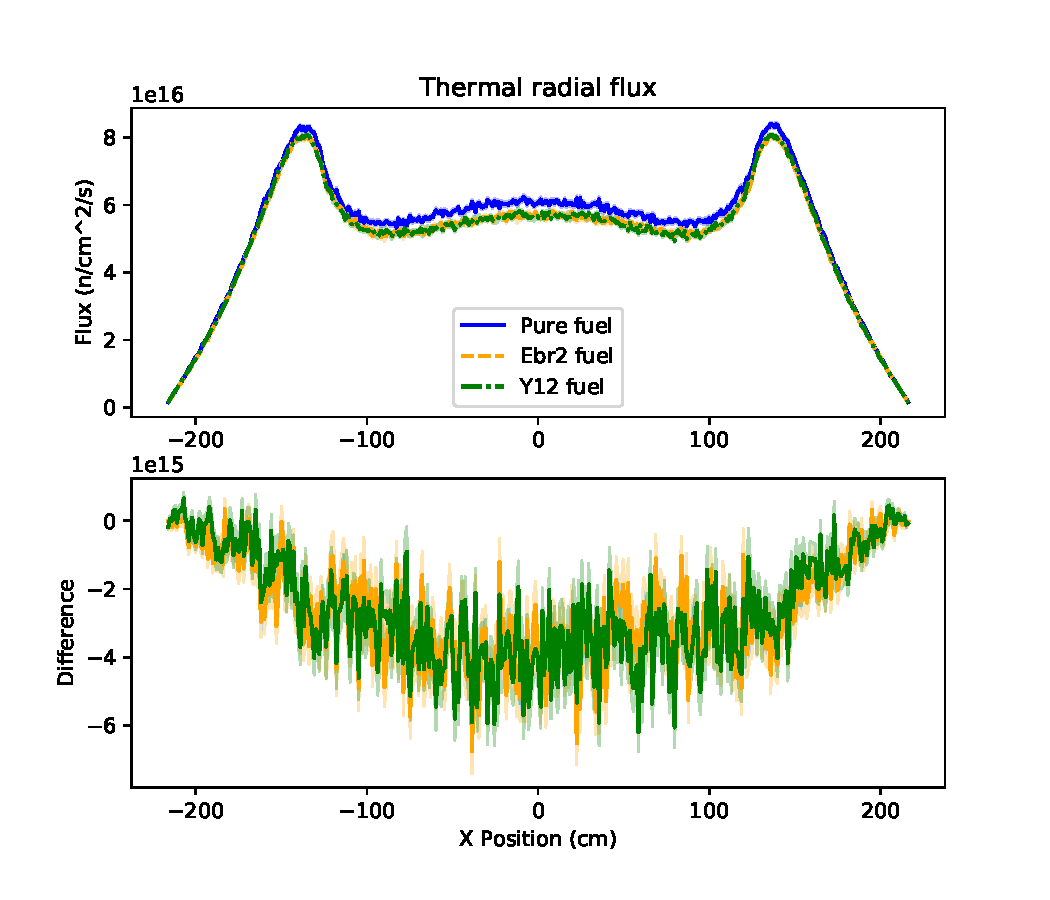
\includegraphics{xe100_thermal_radial.pdf}
        \caption{Thermal flux in the Xe-100-like Sangamon200 
        reactor model in the radial direction, across the 
        x-axis.}
        \label{fig:xe100_thermal_radial}
\end{figure}

\begin{figure}
        \centering 
        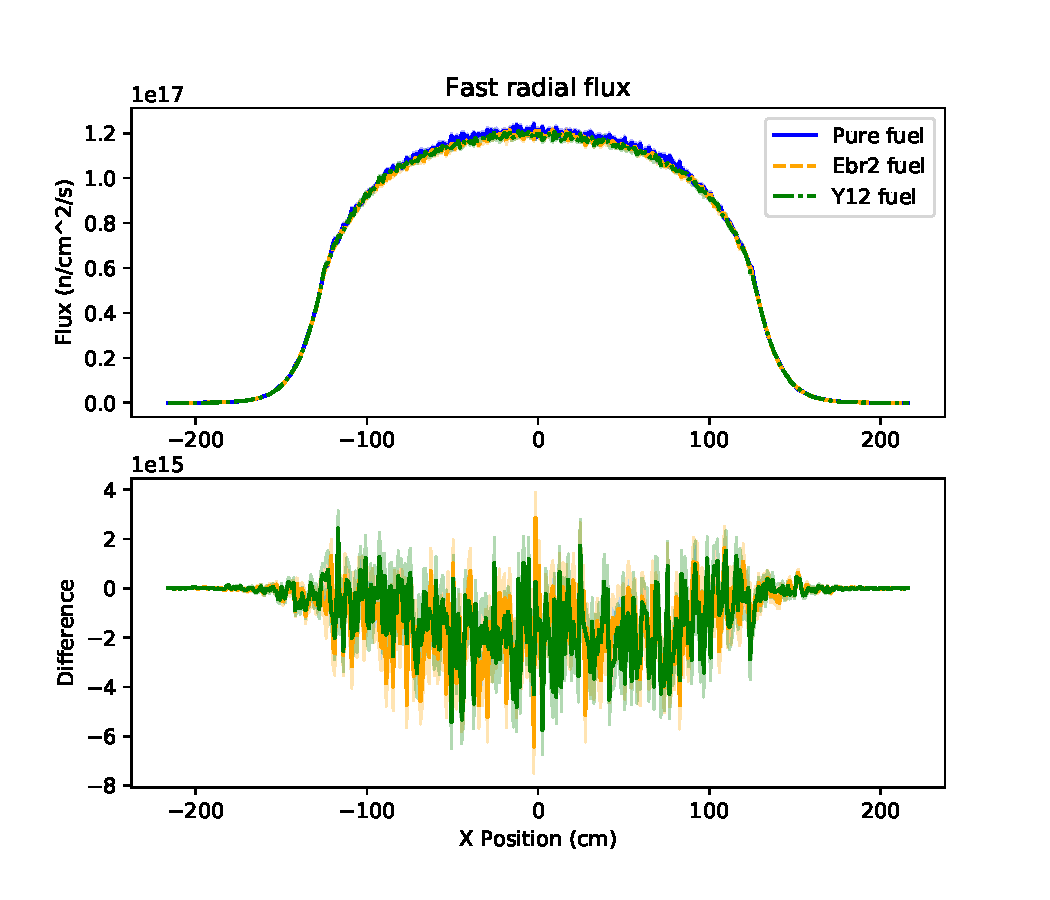
\includegraphics{xe100_fast_radial.pdf}
        \caption{Fast flux in the Xe-100-like Sangamon200 
        reactor model in the radial direction, across the 
        x-axis.}
        \label{fig:xe100_fast_radial}
\end{figure}
\begin{figure}
        \centering 
        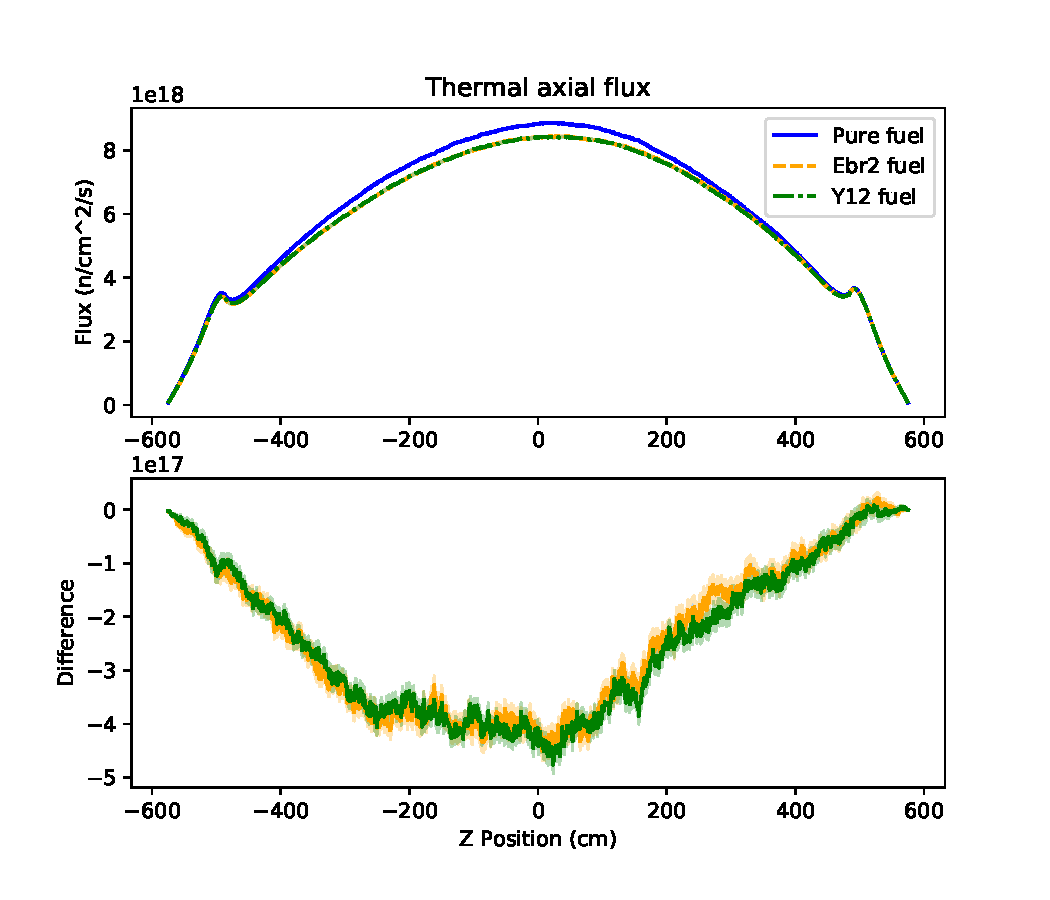
\includegraphics{xe100_thermal_axial.pdf}
        \caption{Thermal flux in the Xe-100-like Sangamon200 
        reactor model in the axial direction.}
        \label{fig:xe100_thermal_axial}
\end{figure}
\begin{figure}
        \centering 
        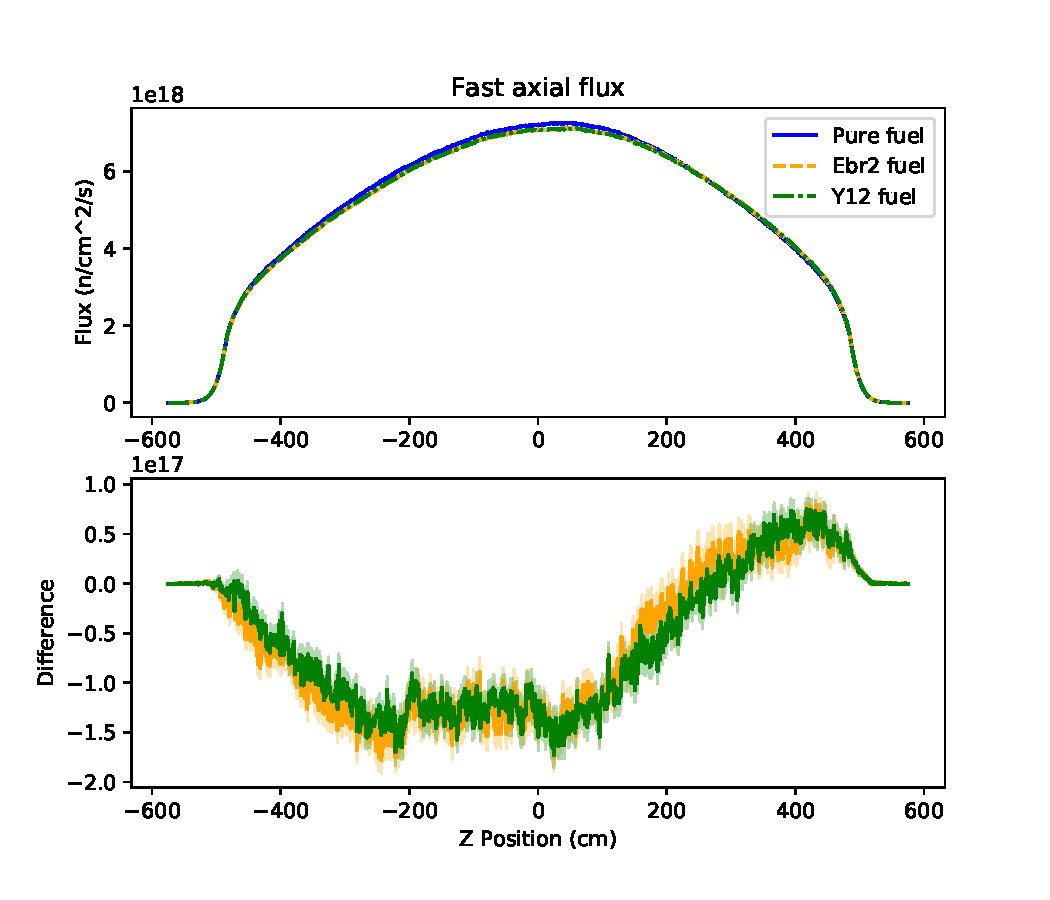
\includegraphics{xe100_fast_axial.pdf}
        \caption{Fast flux in the Xe-100-like Sangamon200 
        reactor model in the axial direction.}
        \label{fig:xe100_fast_axial}
\end{figure}
\subsubsection{Reactivity feedback coefficients}

\begin{table}
        \centering
        \caption{Reactivity temperature feedback coefficients for 
        each material type in the Xe-100-like model for each fuel 
        type.}
        \begin{tabular}{c c c c c}
            \hline 
            & \multicolumn{4}{c}{Material Coefficinet Type} \\
            Fuel Type & Fuel & Coolant & Moderator & Total \\
            \hline
            Pure & -3.875$\pm$0.094 & -0.044 $\pm$ 0.112 & -0.071$\pm$0.459 & -4.216$\pm$0.502\\
            \gls{EBR} & -3.759$\pm$0.138 & -0.433$\pm$0.048 & -0.708$\pm$0.404 & -4.817$\pm$0.438\\
            Y-12 & -3.797$\pm$0.157 & -0.351$\pm$0.092 & -0.728$\pm$0.469 & -4.700 $\pm$0.349\\
            \hline

        \end{tabular}
\end{table}

\subsection{MMR reactor}